\begin{center}
{\Large {\bf Figures}}
\vspace{3cm}
\end{center}


\begin{figure}[h!]
\begin{center}
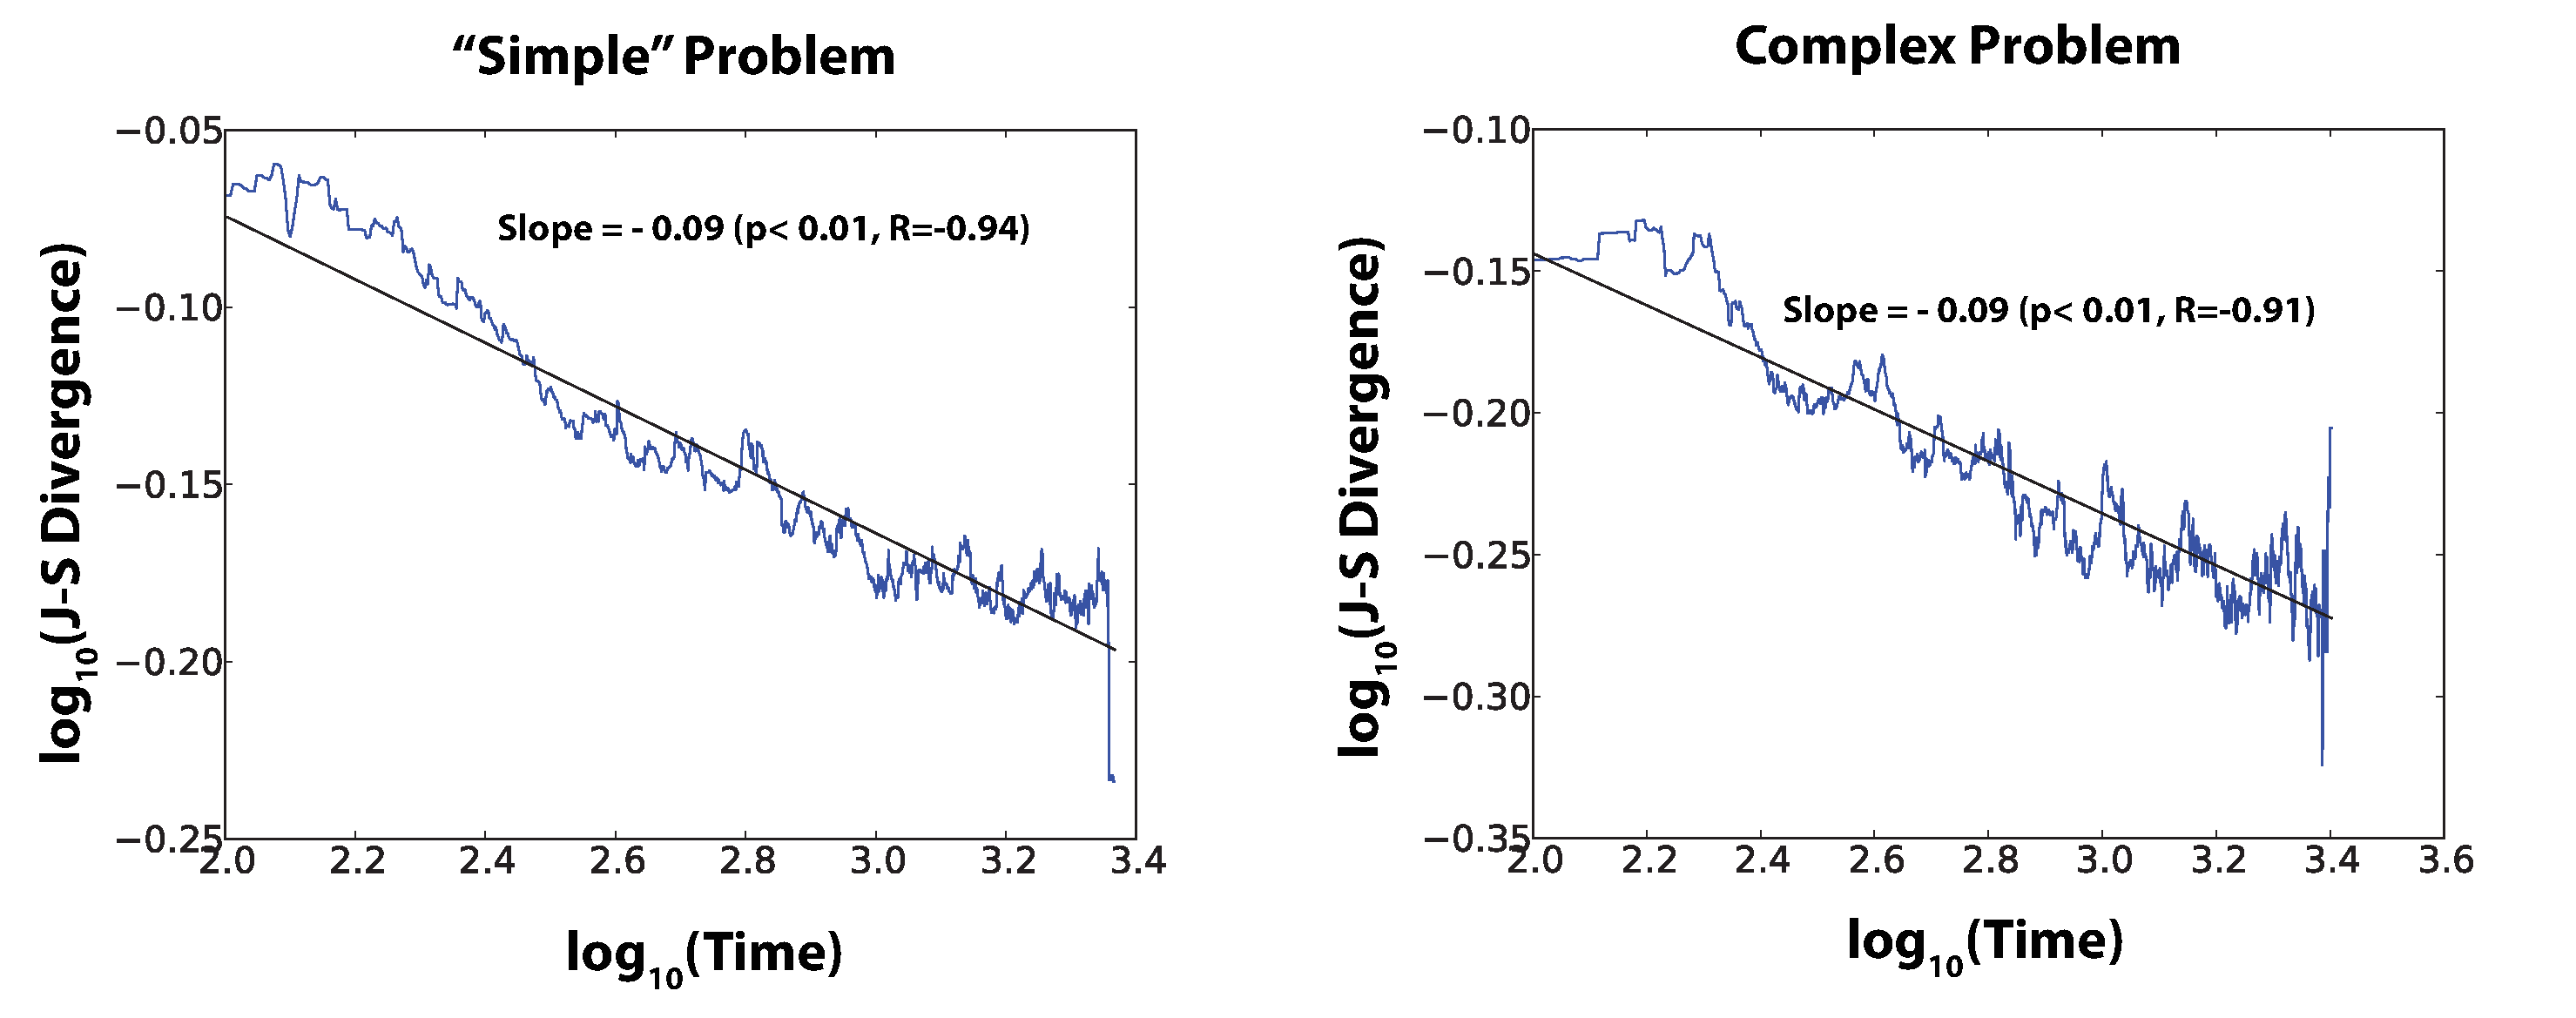
\includegraphics[width=15cm]{figures/ConvergenceMeans.eps}
\caption{Decay of the Jensen-Shannon (JS) Divergence (\ref{JS-divergence}) between models proposed by participants and the true model. The decays are averaged (median or mean?) over all participants in 3-node {\it simple} and 4-node {\it complex} cases (resp. panels {\bf a} and {\bf b}). Both decay follow the same power law decay (\ref{power_law_decay}).}
\label{fig:decay}
\end{center}
\end{figure}

\begin{figure}[h!]
\begin{center}
%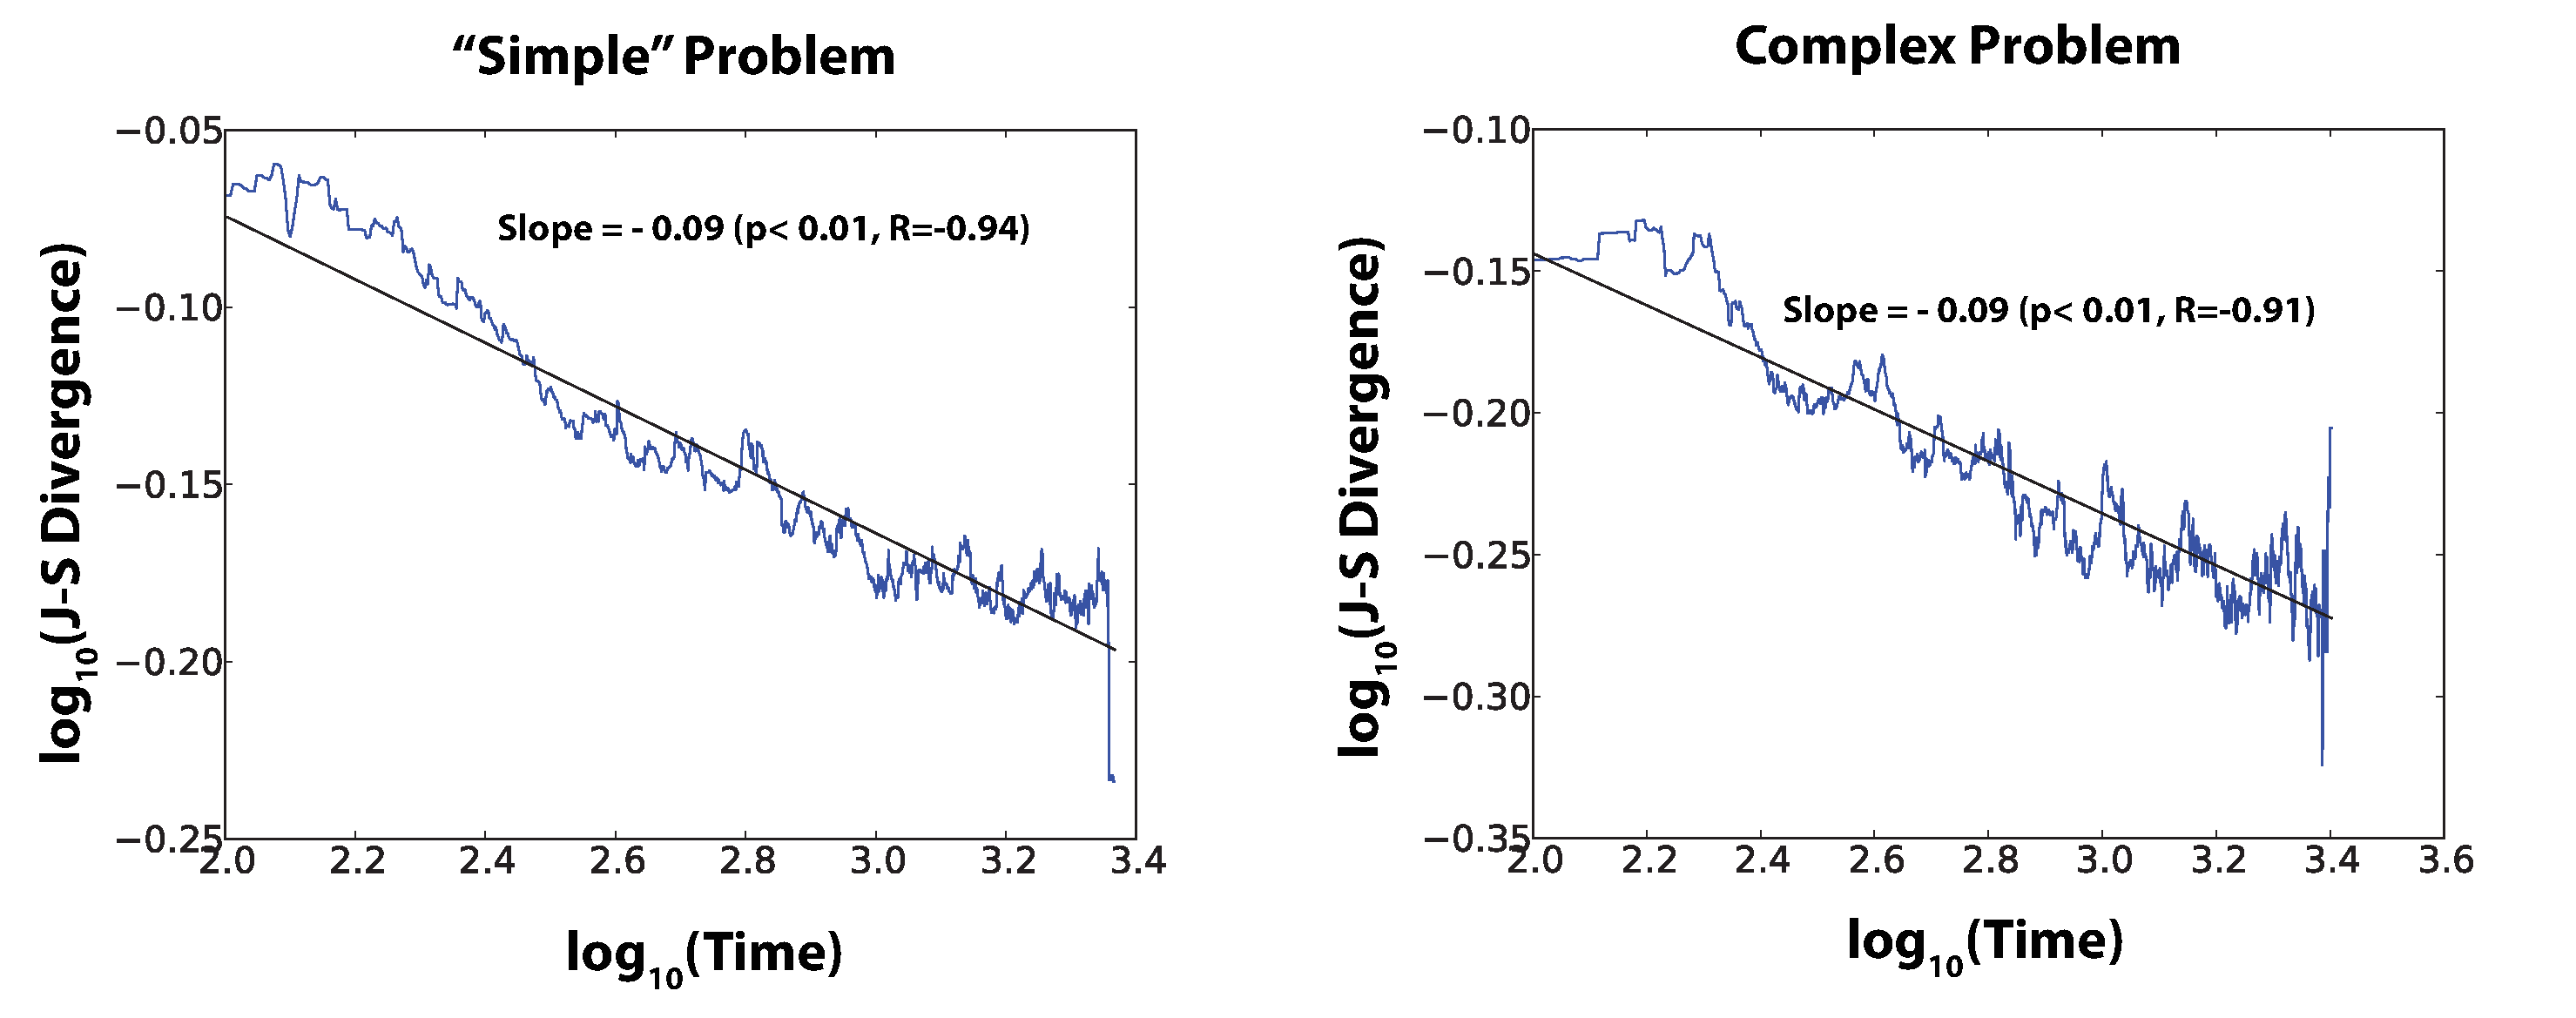
\includegraphics[width=15cm]{figures/ConvergenceMeans.eps}
\caption{Distribution of jump sizes}
\label{fig:jump_sizes}
\end{center}
\end{figure}

\begin{figure}[h!]
\begin{center}
%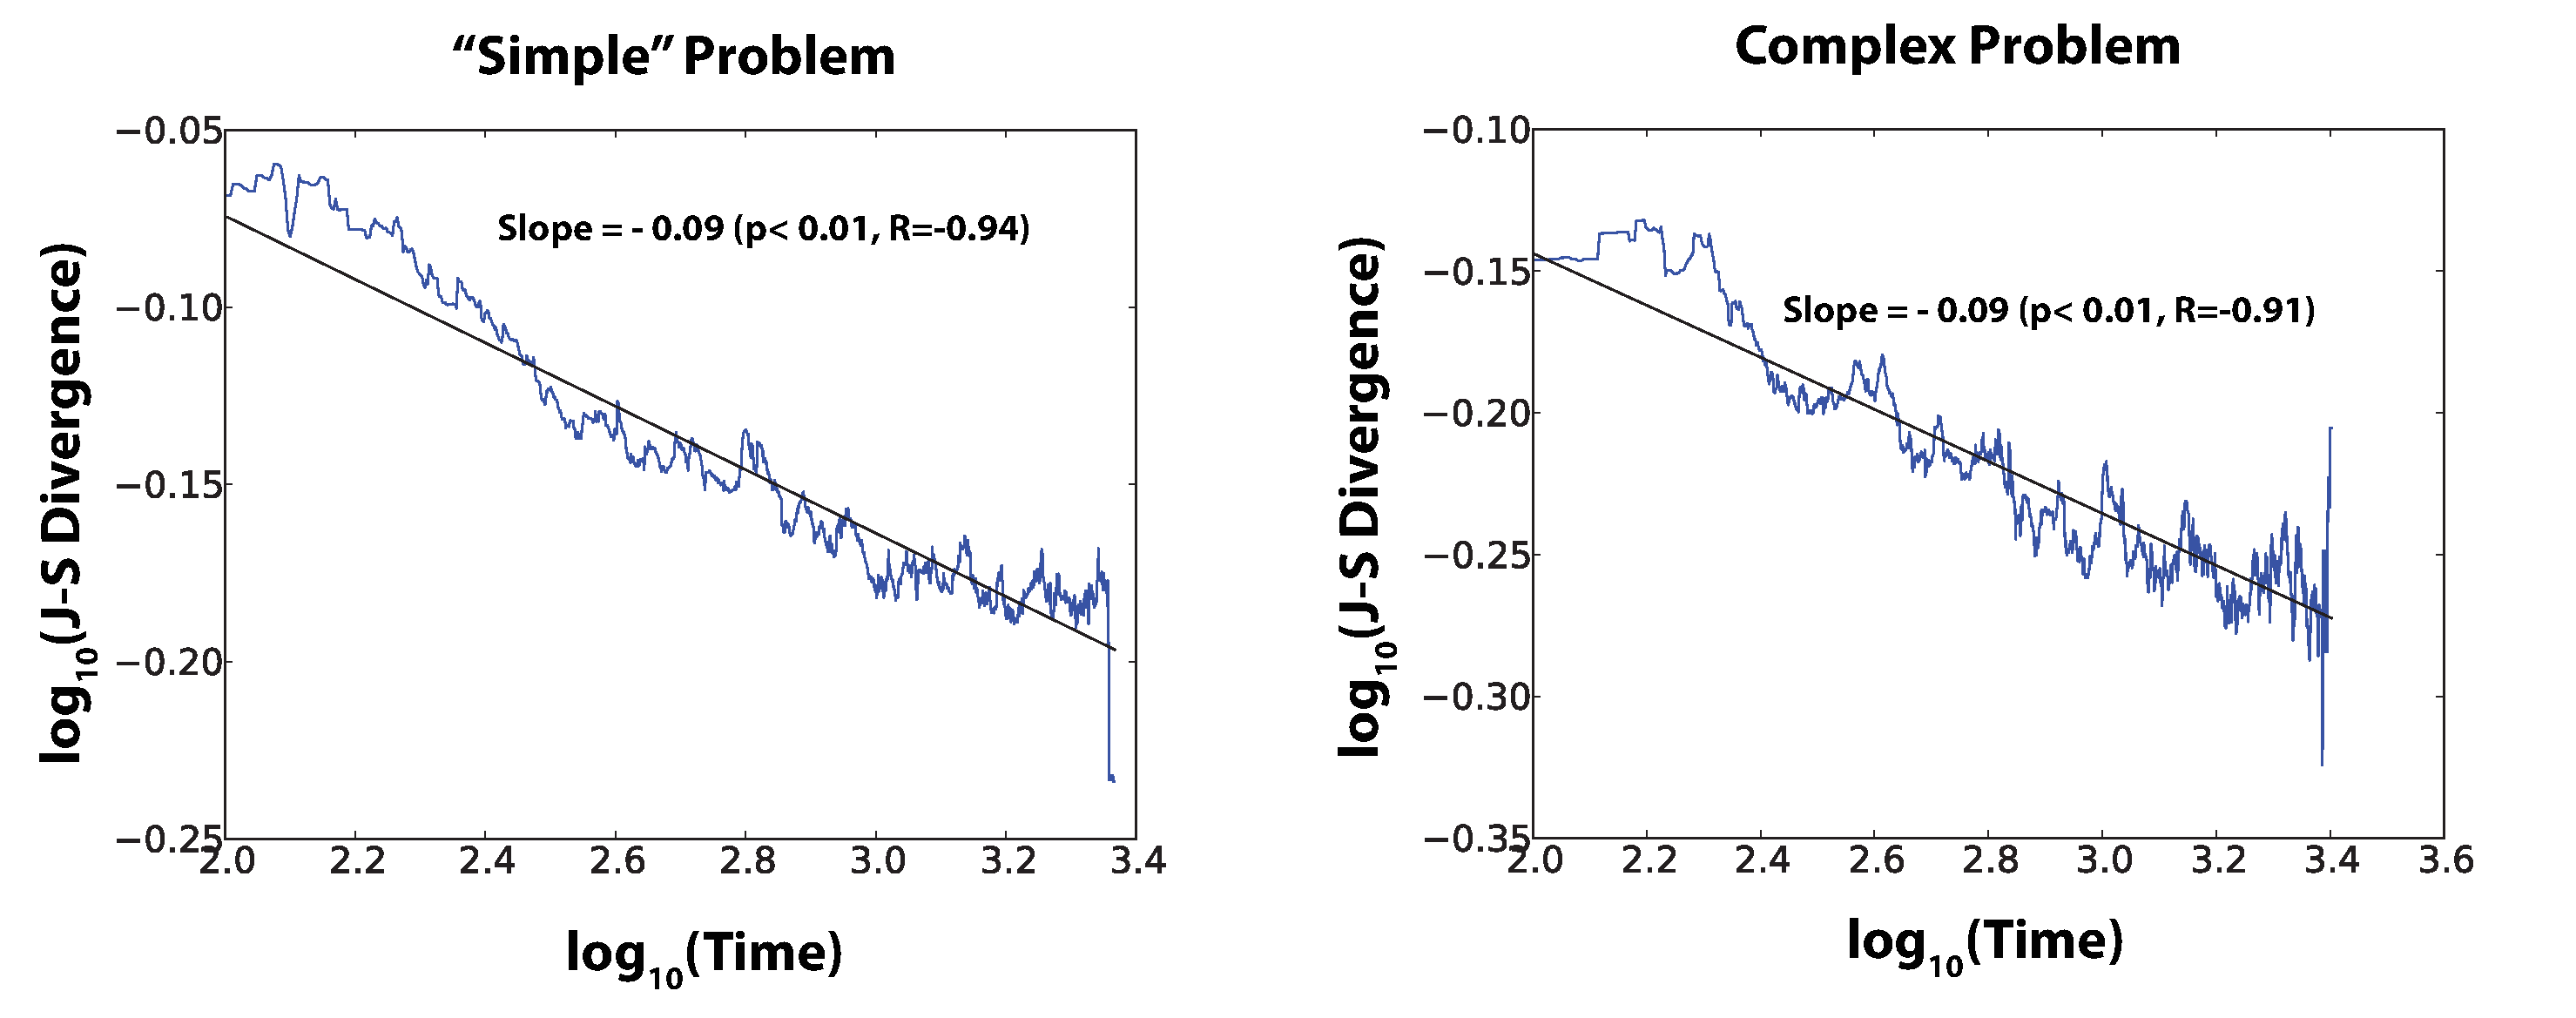
\includegraphics[width=15cm]{figures/ConvergenceMeans.eps}
\caption{Distribution of Waiting Times}
\label{fig:waiting_times}
\end{center}
\end{figure}


\begin{figure}[h!]
\begin{center}
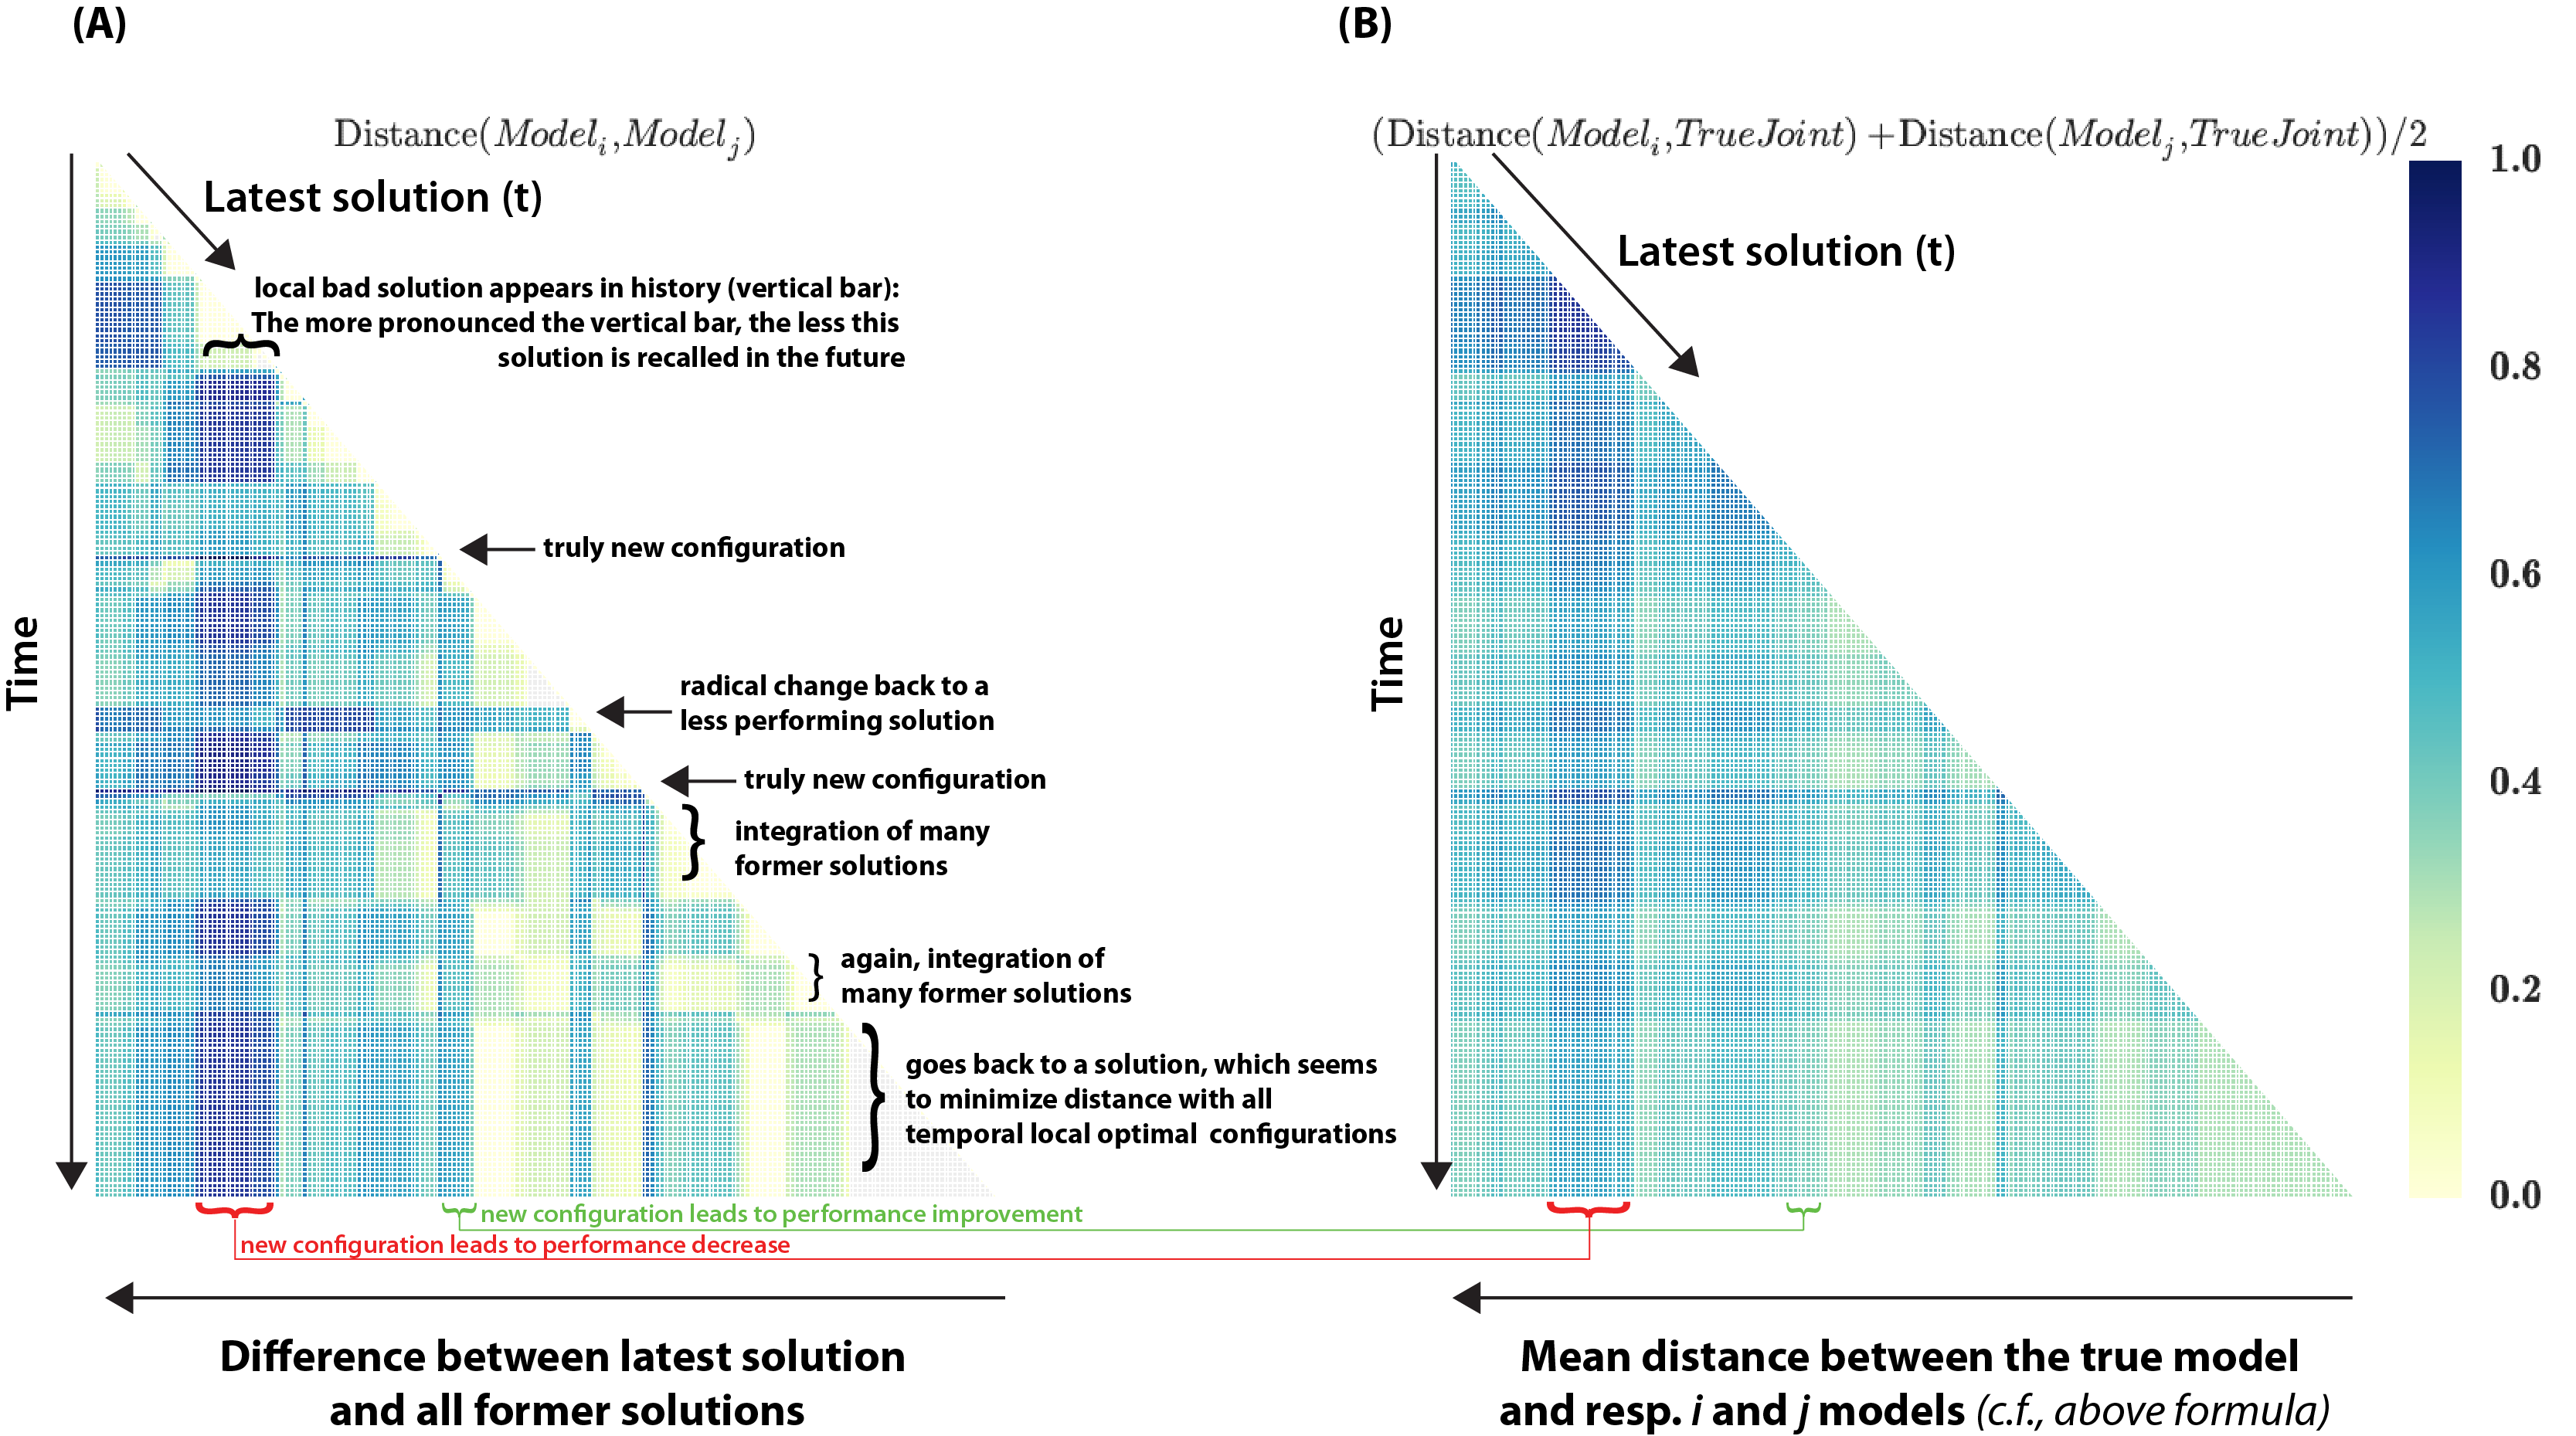
\includegraphics[width=15cm]{figures/matrice2.png}
\caption{\footnotesize Triangular matrices of difference between {\bf A} latest solution as a function of time and all former solutions, and {\bf B} of mean distance between the true model and resp. $i$ and $j$ configurations. Matrix {\bf B} shows the performance of a proposed model and serves as a reference for rationalizing choice sequences made by participants. These choice sequences are represented in matrix {\bf A} for participant 13: We see a wealth of characteristic choices leading to better of worse solutions, but also some integration and disruptive change in strategies, some which having a positive impact on performance, and other having a negative impact on performance. The rectangle structures show that participants do not drastically update drastically, but rather alternate periods of fine tuning and radical innovation. Matrix {\bf A} can also be watched in a more heuristic way at the coarse grained level: The more contrasted the pattern the more innovation overall. And, as shown here for participant 13, as more models are tested -- towards the lower right corner -- colors get more yellowish showing overall convergence of models. In the case presented here, the convergence of models leads overall to better solutions over time. It may not always be the case.}
\label{fig:matrices}
\end{center}
\end{figure}


\vspace{1cm}
\begin{figure}[h]
\label{init_final_best}
%\centerline{\epsfig{figure=../figures/histogram.eps,angle=0,width=14cm,scale=1}}
\caption{How does the initial guess influence the final (resp. best) score?}
\label{figure1}
\end{figure}

